% ****** Start of file apssamp.tex ******
%
%   This file is part of the APS files in the REVTeX 4.1 distribution.
%   Version 4.1r of REVTeX, August 2010
%
%   Copyright (c) 2009, 2010 The American Physical Society.
%
%   See the REVTeX 4 README file for restrictions and more information.
%
% TeX'ing this file requires that you have AMS-LaTeX 2.0 installed
% as well as the rest of the prerequisites for REVTeX 4.1
%
% See the REVTeX 4 README file
% It also requires running BibTeX. The commands are as follows:
%
%  1)  latex apssamp.tex
%  2)  bibtex apssamp
%  3)  latex apssamp.tex
%  4)  latex apssamp.tex
%
\documentclass[%
 reprint,
%superscriptaddress,
%groupedaddress,
%unsortedaddress,
%runinaddress,
%frontmatterverbose, 
%preprint,
%showpacs,preprintnumbers,
%nofootinbib,
%nobibnotes,
%bibnotes,
 amsmath,amssymb,
 aps,
%pra,
%prb,
%rmp,
%prstab,
%prstper,
%floatfix,
]{revtex4-1}

\usepackage{graphicx}% Include figure files

\usepackage{dcolumn}% Align table columns on decimal point
\usepackage{bm}% bold math
%\usepackage{hyperref}% add hypertext capabilities
%\usepackage[mathlines]{lineno}% Enable numbering of text and display math
%\linenumbers\relax % Commence numbering lines

%\usepackage[showframe,%Uncomment any one of the following lines to test 
%%scale=0.7, marginratio={1:1, 2:3}, ignoreall,% default settings
%%text={7in,10in},centering,
%%margin=1.5in,
%%total={6.5in,8.75in}, top=1.2in, left=0.9in, includefoot,
%%height=10in,a5paper,hmargin={3cm,0.8in},
%]{geometry}


%% new commands
\newcommand {\ket} [1] {|{ #1 \rangle}}
\graphicspath{{C:/Users/Steffi/Dropbox/THESIS/T1paper/figures}}

\begin{document}


\title{Electron spin relaxation effects of a single phosphorus donor in silicon at low temperatures}% Force line breaks with \\

\author{Stefanie Tenberg}
 \affiliation{Centre for Quantum Computation and Communication Technology, School of Electrical Engineering \& Telecommunications, UNSW Sydney, New South Wales 2052, Australia.}
 \author{Serwan Asaad}
 \affiliation{Centre for Quantum Computation and Communication Technology, School of Electrical Engineering \& Telecommunications, UNSW Sydney, New South Wales 2052, Australia.}
 \author{Mark Johnson}
 \affiliation{Centre for Quantum Computation and Communication Technology, School of Electrical Engineering \& Telecommunications, UNSW Sydney, New South Wales 2052, Australia.}
 \author{Mateusz Madzik}
 \affiliation{Centre for Quantum Computation and Communication Technology, School of Electrical Engineering \& Telecommunications, UNSW Sydney, New South Wales 2052, Australia.}
\author{Arne Laucht}
 \affiliation{Centre for Quantum Computation and Communication Technology, School of Electrical Engineering \& Telecommunications, UNSW Sydney, New South Wales 2052, Australia.}
\author{Robert Joynt}
 \affiliation{University of Wisconsin-Madison, Physics Department
1150 University Ave, Madison, Wisconsin 53706, USA}
\author{Andrea Morello}
 \email{a.morello@unsw.edu.au}
 \affiliation{Centre for Quantum Computation and Communication Technology, School of Electrical Engineering \& Telecommunications, UNSW Sydney, New South Wales 2052, Australia.}


\date{\today}

\begin{abstract}
We analyse the electron spin relaxation of donors in silicon at low temperatures with external magnetic field and donor confinement depth. For the magnetic field dependence, we observe the predicted $1/T_1\sim B^5$ phonon induced relaxation at magnetic fields $B\gtrsim 2\,$ T for three different samples. We see two orders of magnitude change in the strength of the relaxation however. This is related to the difference in strain in the samples which reduces the matrix elements of the second order phonon process.
Furthermore, for $B\lesssim 2\,$T, the relaxation behaviour changes to $1/T_1\sim B$ for two out of the three samples. This is compatible with relaxation induced through evanescent wave Johnson noise created by the metal structures on top of the donors. 
The donor confinement becomes particularly relevant at long relaxation times. For shallow confinement co-tunnelling increases the relaxation but is suppressed for deep confinements.
Conclusively, we have identified three different aspects limiting the relaxation in donors in silicon which not only gives greater insight into the microscopic picture of this environment but also allows for engineering qubits with improved relaxation times. 
\begin{description}

\item[PACS numbers]
May be entered using the \verb+\pacs{#1}+ command.

\end{description}
\end{abstract}

\pacs{Valid PACS appear here}% PACS, the Physics and Astronomy
                             % Classification Scheme.
%\keywords{Suggested keywords}%Use showkeys class option if keyword
                              %display desired
\maketitle


\section{\label{sec:introduction}Introduction}

The electron spin-lattice relaxation time $T_1$ in donors in silicon is of great interest. Not only gives it insight into the fundamental physics of the system but also is extremely relevant for donor spin qubits which have proven to be excellent candidates for quantum computation \cite{Muhonen2014, Muhonen2015}. Indeed the qubit coherence times of up to $T_2=1\,$s approach the limit set by the relaxation time \cite{Kalra2016}. However, few experiments have been performed on to learn more about the mechanisms reducing $T_1$. 

Generally, relaxation happens due to fluctuations in the transverse elements of the Hamiltonian at the Larmor frequency of the spin states. This requires the spin to be coupled to a phonon reservoir.
As silicon is not a piezoelectric material this coupling is only achieved by the deformation potential. Phonons, in form of acoustic waves, deform the lattice while travelling through the crystal. This breaks the 6 fold symmetry which in turn shifts the energy bands by a  magnitude defined by the deformation potential. The relative valley population changes causing a shift in the g-factor. This shift oscillates with the phonon frequency and relaxes the spin \cite{Hasegawa1960}. Furthermore, local strain couples the gamma and delta energy bands in one valley, effectively changing the g factor locally and thus also relaxing the spin in the same fashion \cite{Roth1960}. 
This spin-lattice relaxation can be described by 
\begin{eqnarray}\label{eq:fullT1}
T_1^{-1} & = & \frac{1}{90\pi k_B}\left(\frac{g_{||}-g_\perp}{g_0}\right)\left(\frac{\Xi_u}{E_{12}}\right)^2\\
& &\left(\frac{1}{\rho \bar{v}_t^5}+\frac{2}{3\rho\bar{v}_l^5}\right)\left(\frac{g_0\mu_0B}{\hbar}\right)^5f(\theta)
\end{eqnarray}
in the high temperature limit where $\frac{g_{||}-g_\perp}{g_0}$ is the anisotropy in the g-factor, $\Xi_u$ is the deformation potential, $E_{12}$ is the valley orbit splitting between the ground and first excited state, $v_l, v_t$ are the sounds velocities in silicon, $\rho$ is the density of silicon and $f(\theta)$ is an angular factor with regard of the external magnetic field $B_0$ and the crystal axis \cite{Wilson1961}.
At low temperatures only spontaneous phonon emission is possible so that a $T_1\sim B^5$ dependence with magnetic field is expected \cite{Morello2010, Zwanenburg2013}. 

Previously the dependence of $T_1$ on external magnetic field at low temperatures of donors in silicon has been measured by Morello \textit{et. al.} \cite{Morello2010} on two single phosphorus donors in a CMOS style device and Watson \textit{et. al} \cite{Watson2015} on a single phosphorus donor in a STM hydrogen lithography device. While two of these three measurements conform with each other and follow the expected $T_1\sim B^5$, one measurement by Morello \textit{et. al.} shows a strong deviation. Not only is the magnitude of the $B^5$ relaxation one order of magnitude different but also deviates the measurement from $T_1\sim B^5$ to $T_1\sim B$ at low magnetic fields $B<2\,$T.  

In this paper we add two detailed measurements of the relaxation with magnetic field in enriched silicon $^{28}$Si. We analyse the causes for the differences in behaviour of those measurements to extend the understanding of relaxation in silicon donor devices. 

Furthermore, as the relaxation time approaches multiple seconds, we observe effects of the electro-statical environment on the relaxation. Thus, to complete this picture, we study the relaxation with both donor confinement depth (plunge voltage) and SET electron number. 

This study revealed three different effects that influence the relaxation time in this system:  Firstly, we observe an effect that leads to a dominant $T_1\sim B$ dependence of the relaxation time at low magnetic fields. This dependence is conclusive with a relaxation caused by Evanescent wave Johnson noise (EWJN).
% EWJN relaxes the donor electron by stimulated emission into the enhanced density of states of the electromagnetic waves decaying from the Aluminium structures on top of the donor.
 Secondly, strain strongly suppresses the phonon relaxation. Lastly, co tunnelling decreases the $T_1$ if the donor is not plunged deep enough below the Fermi level.
 % The $\ket{\uparrow}$ electron escapes from the donor through a virtual co-tunnelling process into free states of the reservoir of the SET island and is replaces by $\ket{\downarrow}$. The tunnel rate strongly depends on the depth of the donor level beneath the Fermi level. Thus it can be mitigated by pulsing deeply below the Fermi level during operation.

The remainder of this paper will show and explain these results and is organised as follows. Section \ref{sec:background} explains our physical system and the experimental set up as well as the measurement techniques. Then section \ref{sec:extB} shows the results of the magnetic field dependence measurements where we both analyse the low magnetic field behaviour in section \ref{sec:ewjn} and the high magnetic field behaviour in section \ref{sec:strain}. Lastly, section \ref{sec:cotunnelling} presents the electrostatic environment measurements. Finally, section \ref{sec:conclusion} discusses the results, open questions and possible future measurements. 


\section{\label{sec:background} The qubit system and measurement methods}

\begin{figure}
\centering
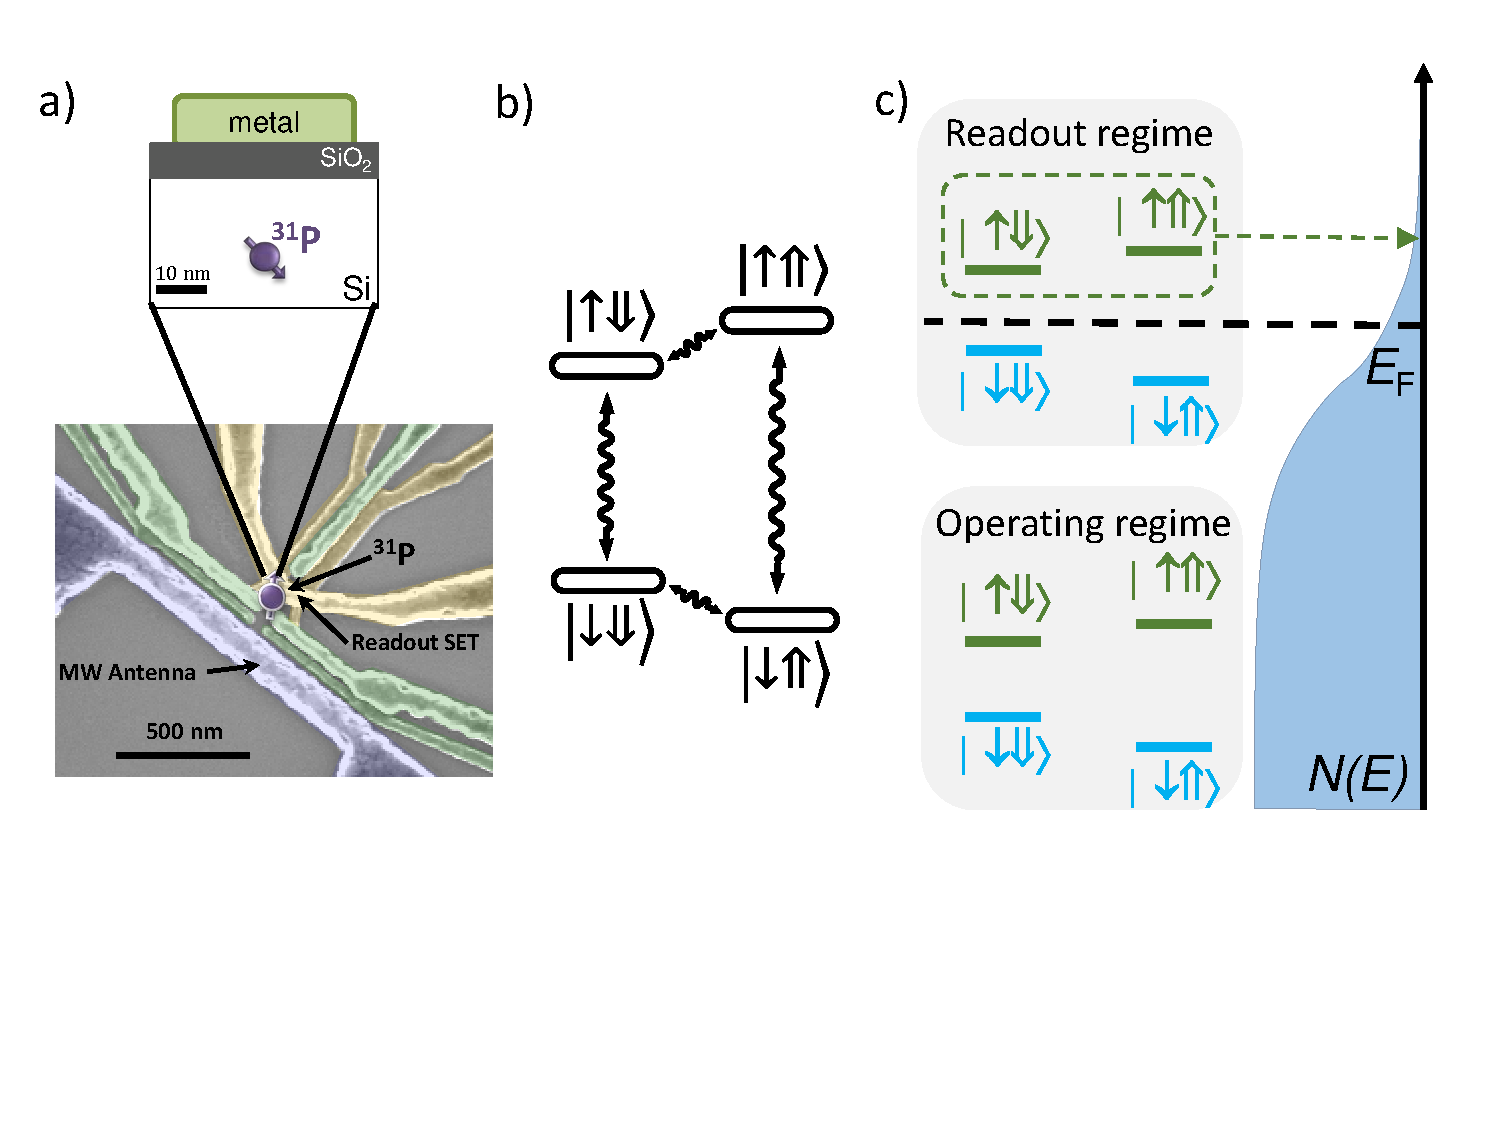
\includegraphics[width=\columnwidth]{fig1.pdf}
\caption{
(a) Schematic of a phosphorus donor implanted in enriched $^{28}$Si with a scanning electron micrograph of an identical device to the one measured. Four gates control the donor potential while a single electron transistor (SET) detects electron tunnel events in its environment to determine the qubit state. A broadband microwave antenna provides an electromagnetic drive for both the electron and the nucleus. b) Energy diagram of the electron-nuclear spin system, with ESR and NMR transitions indicated. (c) Schematic of the two regimes the donor qubit is operated in for the relaxation measurements: 1. Readout regime, where the Fermi level of the SET reservoir is tuned such that $\ket{\uparrow}\rangle$ can tunnel out, producing a current spike, while $\ket{\downarrow}$ stays confined, keeping the current low. 2. Operating regime, where both spin states are well confined below the Fermi level.
}
\label{fig:device}
\end{figure}

Our qubit is a single electron spin confined by a phosphorus $^{31}$P donor implanted in enriched $^{28}$Si as shown in the schematic in figure \ref{fig:device} (a). An external magnetic field is applied to separate the spin states into a well defined two level system. This leads to a two-qubit system: The donor electron with $S=1/2$ and basis states $\ket{\uparrow},\ket{\downarrow}$ and the $^{31}$P nucleus with $I=1/2$ and basis states $\ket{\Uparrow},\ket{\Downarrow}$. The energy levels of this system are displayed in figure \ref{fig:device} (b). Aluminium gates on top of the donor control the electrostatic environment and are used to apply DC pulses while a broadband microwave antenna is used for microwave and radio frequency pulses. This gives full control over the qubit states. A nearby single electron resistor (SET) allows for tunnelling into its reservoir with an electron temperature of $T\approx 100\,$mK. It acts as a readout mechanism for the electron by detecting its charge tunnelling events into the reservoir. A scanning electron micrograph of the device is shown in figure \ref{fig:device} (a). This paper focusses on the electron qubit only. For the experiments in this paper this qubit is operated in two regimes: Firstly, the readout regime, where the donor is tuned such that $\ket{\uparrow}$ tunnels to the reservoir of the SET while $\ket{\downarrow}$ stays confined. This allows for single shot readout. Secondly, the operating regime, where the donor is tuned such that both electron spin states lie well below the Fermi level of the SET. These regimes are illustrated in figure \ref{fig:device} (c). 


\subsection{\label{sec:Measurementprocedures} Measurement procedures}

\begin{figure}
\centering
\includegraphics[width=\columnwidth]{fig2.pdf}
\caption{
(a) Schematic of the pulse sequence used in the experiments. The solid line represents the position of the donor energy levels with respect to the Fermi level achieved by the combined voltages of the donor gates. For fields $B_0\leq1.5\,$T $\ket{\downarrow}$ is initialized and then inverted to achieve higher contrast while for $B>1.5\,$T a random load is performed. (b) Example of a $T_1$ measurement at $B=1.5\,$T. The relaxation time is extracted by a least-square fit to $T_1=3.7\pm0.4\,$s.
}
\label{fig:t1example}
\end{figure}

To determine the relaxation time $T_1$ of the electron we repeatedly measure the $\ket{\uparrow}$ proportion after a period of time $\tau$ has elapsed while the donor is in the operating regime.  The applied pulse sequence is illustrated in figure \ref{fig:t1example} (a). First, we initialize the electron in the $\ket{\downarrow}$ for external magnetic fields of $B_0<1.5$T. We wait for roughly the tunnel time in the readout regime so that the $\ket{\uparrow}$ tunnels into the reservoir and is replaced by $\ket{\downarrow}$. If a high precision is required to increase the measurement contrast, we apply a technique called Bayesian update. A feedback loop is applied that self-corrects for wrongly loaded $\ket{\uparrow}$ and can achieve initialization fidelities of over $99\%$ \citep{Johnson2018}. After initialization, $\ket{\downarrow}$ is inverted to $\ket{\uparrow}$ by applying an electron spin resonance $\pi$ pulse. Then the donor remains for time $\tau$ in the operating regime at plunge depth $V_{p}$. Lastly, a single shot readout is performed in the readout regime. Figure \ref{fig:t1example} (b) shows an example measurement of the relaxation time at $B_0=1.5$T. The $T_1$ time is extracted by performing a least-square fit. For $B_0>1.5\,$T a random load is performed by simply emptying and reloading an electron, thus preparing either $\ket{\uparrow}$ or $\ket{\downarrow}$ randomly. The remainder of the pulse sequence is the same. The plunge voltage $V_p$ is created by biasing two of the donor gates and the SET top gate together, changing the chemical potential of the donor electron with respect to the Fermi level of the SET island. Unless otherwise stated, these pulses are compensated which means that the SET Fermi level is kept constant while moving the donor. 



\section{\label{sec:extB}Relaxation time dependence on external magnetic field}

\begin{figure}
\centering
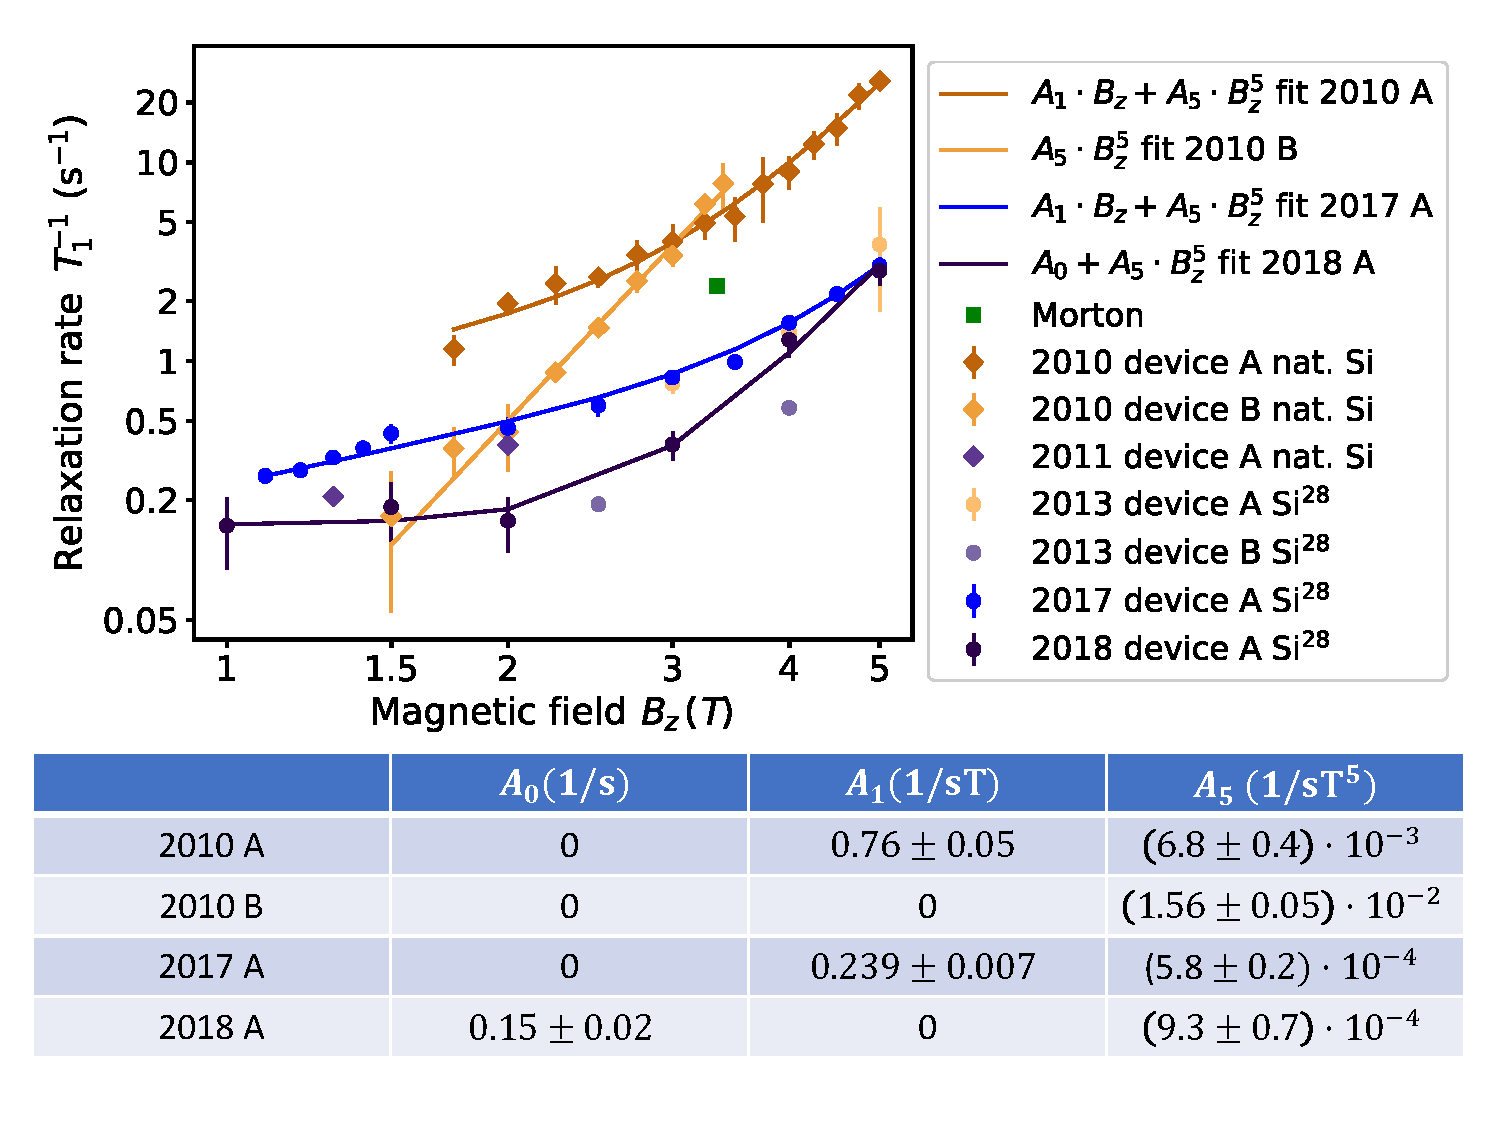
\includegraphics[width=\columnwidth]{fig3.pdf}
\caption{
MATEUSZ DATA STILL TO INCLUDE. (a) Measurements of the dependence of electron spin-lattice relaxation time $T_1$ on the external magnetic field $B_0$ from different samples. Device 2010A and 2010B are taken from \cite{Morello2010} and are natural silicon, same as device 2011A. Device 2017A and 2018A have been measured on Si$^{28}$, as have devices 2013A and B. For device 2010A, B, 2017A and 2018A curves of form $A_1B_0+A_5B_0^5$ have been fitted. (b) Fit results of the different samples. 
}
\label{fig:magnetic field dependence}
\end{figure}


In this section we are analysing the dependence of the relaxation time on the strength of the external magnetic field $B_0$. Figure \ref{fig:magnetic field dependence} (a) shows full sets of relaxation rates with magnetic field for four donor qubits with almost identical device layout: sample 2010A and 2010B which are  natural silicon samples, taken from \cite{Morello2010}, and samples 2017A and 2018A which are enriched Si$^{28}$ samples. Furthermore, small measurement sets of three more qubits are displayed. 
Both device 2010A and 2017A show a strong deviation from the expected $T_1\sim B^5$ and instead behave linearly below $B\approx 2.5\,$T. We fit $A_1B_0+A_5B_0^5$ to those curves and $A_5B^5$ to device 2010B to quantify their behaviour. The fit results are shown in table \ref{fig:magnetic field dependence} (b). The cause for this linear behaviour is presented in the next sub section.

\subsection{\label{sec:ewjn}Evanescent wave Johnson noise}

\begin{figure}
\centering
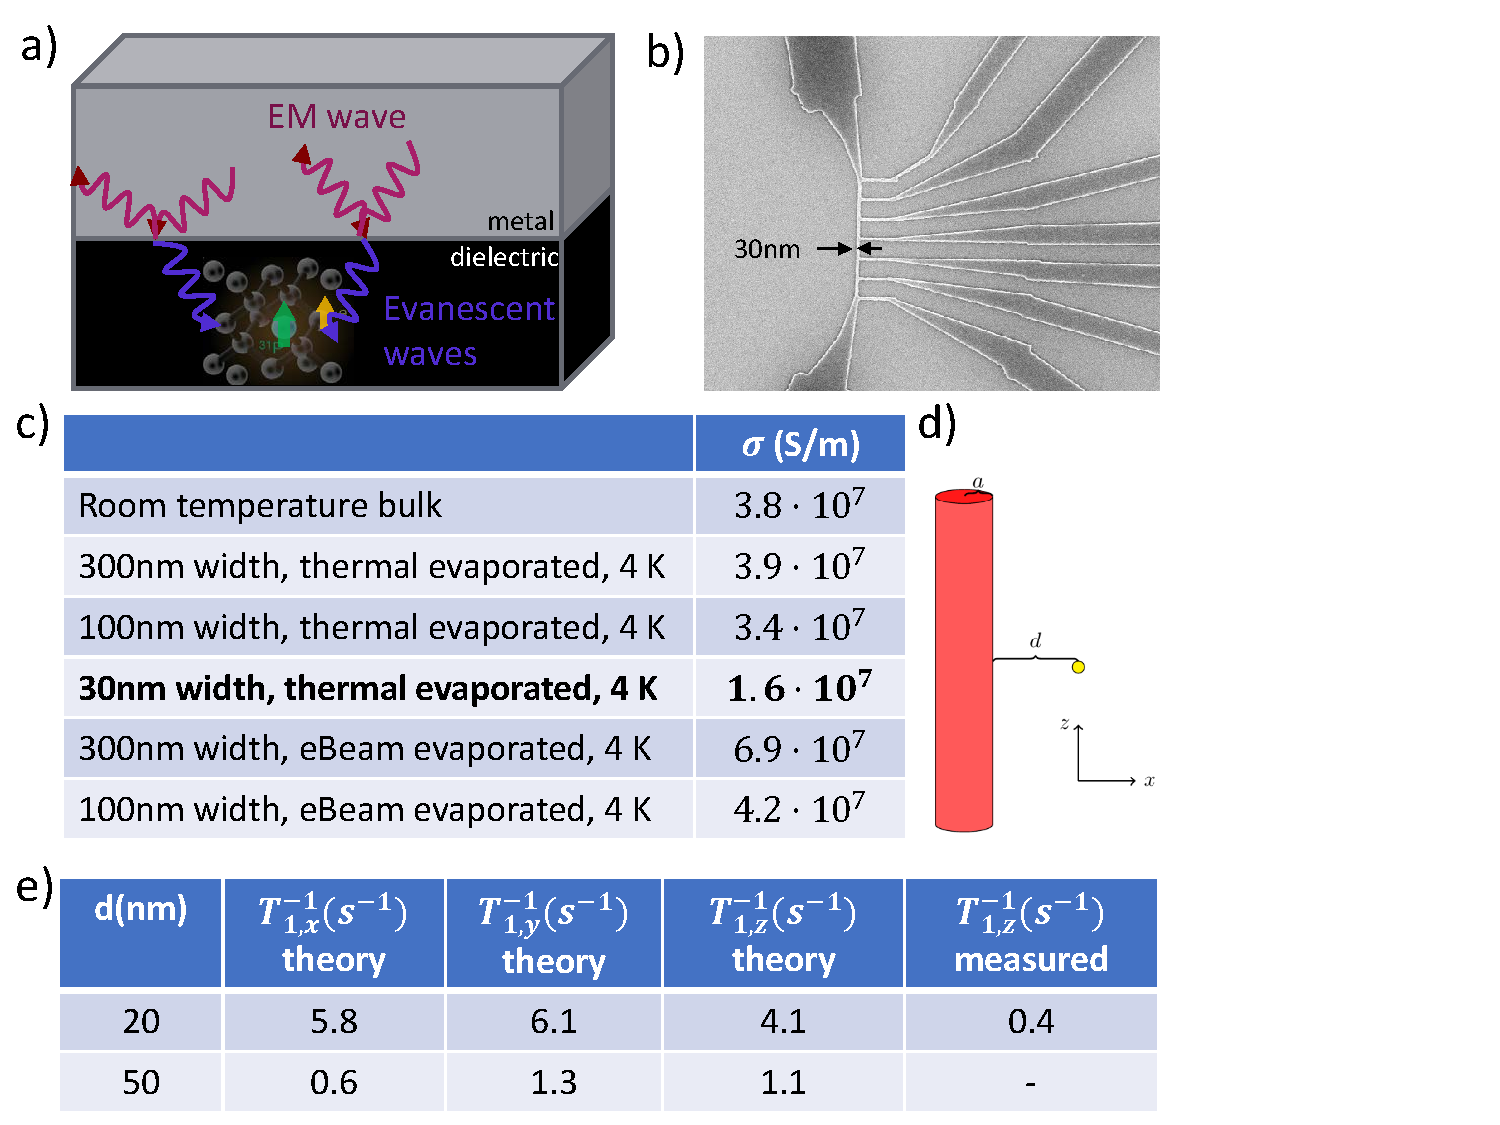
\includegraphics[width=\columnwidth]{fig4.pdf}
\caption{
(a)Schematic of the origin of evanescent wave Johnson noise in our qubit devices. (b) Scanning electron micrograph of a Hall bar structure with feature size of $30\,$nm. (c) Table of conductance values for different feature sizes and evaporation techniques of Aluminium devices. 
Aluminium thickness is 50nm. (d) Geometry assumption for theoretical calculations where the cylinder represents the metal gate on top of the qubit with diameter $a$ and distance $d$. (e) Table of relaxation rates predicted by the EWJN theory and measured values. 
}
\label{fig:ewjn}
\end{figure}

Our qubits are in the vicinity of metal electrodes that contain mobile charges and spins. The thermal and quantum motion of these creates random electromagnetic fields that decohere and relax the qubit. This we know as Johnson noise. It leaks out of the metal into the insulator in form of evanescent waves when the photons are reflected on the metal-insulator interface. Thus there is strong Johnson noise near the metallic surface which is called evanescent wave Johnson noise (EWJN) \cite{Premakumar2017}. At low temperatures this can lead to relaxation as it enhances the density of available states to the donor electron and thus stimulates emission. For this type of magnetic noise that couples directly to the electron spin, we can always write the relaxation rate as

\begin{equation}
T_1^{-1}=\frac{1}{\mathcal{L}}\frac{\mu_B^2\sigma\omega_0}{\hbar c^2}
\end{equation}

where $\mathcal{L}$ is a geometric factor that depends on the geometry of the device, $\sigma$ is the conductivity of the metal structures and $\omega_0$ is the Larmor frequency of the qubit which depends on the magnetic field $\omega_0=\frac{g_0\mu_B B_0}{\hbar}$.  Thus the relaxation follows $T_1^{-1}\sim B_0$. For this theory to be valid, the skin depth $\delta=\sqrt{\mu_0\mu_R\sigma\omega_0/2}^{-1}$ has to be large compared with the dimensions of the metallic elements of the device and the distance of the qubit from those objects. Furthermore, the conduction in the electrodes has to be in the diffusive regime where the mean free path $l_F=v_F\frac{m_e}{ne^2}\sigma$ is much shorter than the device dimensions.  

As the conductance of the aluminium structures directly relates to both the validity of the model through the characteristic length scales and the resulting magnitude of the relaxation, we carefully measure it with 4-point measurements on Hall-bar structures with feature sizes varying from $300\,$nm to $30\,$nm for both thermal and ebeam evaporation. Figure \ref{fig:ewjn} (b) shows a scanning electron micrograph of a $30\,$nm device while table \ref{fig:ewjn} (c) shows the resulting conductance values for all measured structures as well as the standard room temperature bulk value. 
We find that the conductivity drops with reduced feature size but only up to a factor of 2. We choose the 30nm thermal measurement $\sigma=1.6\cdot 10^7\,$S/m for further calculations as this resembles most closely the qubit device measured. This results in $\delta=752\,$nm and $l_F=19\,$nm. Thus, while the skin depth is sufficiently large, the mean free path is comparable with our feature size of around 30nm. This means that we are on the brink between the ballistic and diffusive regime which might reduce the EWJN slightly.

We calculated the geometric dependence according to our device geometry by assuming a conducting cylinder of diameter $a$ and distance $d$ from the qubit as shown in figure \ref{fig:ewjn} (d) and get relaxation rate predictions of 
\begin{eqnarray}
T_1 
\end{eqnarray} 
MORE THEORY STUFF FROM BOB HERE

Putting in our experimental parameters, EWJN predicts relaxation rates as shown in table \ref{fig:ewjn} (e). We find our theory to disagree with our measurement by around one order of magnitude. It is puzzling that the theory predicts a much stronger decay then we observe. 
Another interesting fact is that device 2010B does not exhibit this behaviour, at least not significantly at the magnetic fields that where measured. 

\subsection{\label{sec:strain} Strain dependence}

\begin{figure}
\centering
\includegraphics[width=\columnwidth]{fig7}
\caption{
strain field dependence
}
\label{fig:strain}
\end{figure}

Besides the linear deviation due to EWJN at low fields, our relaxation measurements also show a striking difference in magnitude for the phonon induced relaxation at high fields. All but two devices show a different relaxation coefficient of up to two orders of magnitude as we can see in figure \ref{fig:magnetic field dependence} and table \ref{fig:magnetic field dependence}. 
We relate this to the change in the energy bands due to different amounts of strain in the various samples. Strain arises due to the different lattice constant of Aluminium and silicon. While the energy splitting between the ground and the first excited state does diminish with strain and thus would increase the relaxation rate according to equation \ref{eq:fullT1}, the matrix element of the second order process of acoustic phonons between these states decreases much more dramatically, causing an overall reduction of the relaxation rate.
Figure \ref{fig:strain} shows a simulation of the dependence of the relaxation rate on strain which agrees well with our measurements. Further supporting our argument is the fact that in the STM hydrogen lithography device by \cite{Watson2015} the same relaxation was measured as in device 2010B. The STM device is assumed strain less as there are no metal gates anywhere close to the donor. We speculate that device 2010B was a deep donor , relatively far away from the Aluminium gates. This would also explain the lack of EWJN. Unfortunately, we cannot confirm the donor position in retrospect. Furthermore, we know from previous measurements \cite{Laucht2015} that device 2017A is strained. 



\section{\label{sec:cotunnelling}Co-tunnelling effects}

To analyse the dependence of the relaxation time on the electrostatic environment we start by measuring the relaxation at different donor plunge voltages. The plunge voltage depth and direction determines how far the donor electron spin states are below the Fermi level. 
Usually, for electrons to be able to tunnel between the donor and the SET, they have to conserve energy. However, due to the Heisenberg uncertainty principle, energy conservation can be broken for a time $t_H\approx\frac{\hbar}{E_c}$, where $E_c$ is the confinement of the electron. In this time frame, tunnel effects can appear which relax the donor spin. First order tunnelling (direct tunnelling) is described by 

\begin{equation}\label{eq:directt}
\Gamma = \Gamma_0\cdot e^{-\beta V_p}\cdot\left(1+e^{-{e\alpha V_p}/{k_B T}}\right)^{-1}
\end{equation}
where $\Gamma_0$ is the tunnelling rate from the donor to the SET island when the energy of donor is aligned with SET Fermi level, $\beta$ is the decay factor with plunge voltage, $\alpha$ is the lever arm of the gate voltages to the qubit and $T$ is the electron temperature of the SET electron reservoir \cite{MacLean2007}. This tunnel process is exponentially suppressed with the donor distance to the Fermi level and is only expected as long as at least one donor spin state is above the Fermi level. 

Second order tunnelling (co-tunnelling) is described by 

\begin{equation}\label{eq:cot}
\Gamma = \Gamma_0 \cdot \frac{1}{V_p^2}.
\end{equation}
This tunnel process is also suppressed with donor distance but less strongly and remains possible way below the Fermi level. 

\begin{figure}
\centering
\includegraphics[width=\columnwidth]{fig5.pdf}
\caption{
(a) Charge stability diagram with the donor charge transition indicated in white. The green points represent the compensated plunging, where we move along the SET Coulomb peak so that the SET Fermi level is kept constant while the donor is plunged. The blue points are uncompensated plunging so that we can achieve deeper confinement in the plunge stage. (b) Relaxation rates with plunge voltages, both uncompensated and compensated. The square indicates the region we show zoomed in in (d). (c) Read level voltages varied with plunge voltage to determine the Zeeman splitting through the spin tail. (d) Zoomed in plot for low plunge voltages with Zeeman energy marked and and exponential fit. 
}
\label{fig:plungedependence}
\end{figure}

In figure \ref{fig:plungedependence} we present the measurements of the relaxation time for different donor plunge depths obtained with the method described in section \ref{sec:Measurementprocedures}. Figure \ref{fig:plungedependence} a) shows the measured donor plunge points with respect to the SET Fermi level (dotted line) in the charge stability diagram. We both measure along the Coulomb peaks of the SET, keeping the SET energy constant (green points), as well as perpendicular to it, achieving very deep plunge amplitudes (blue points). In figure \ref{fig:plungedependence} b) the corresponding relaxation rates are plotted where the plunge voltages are normalized to the distance to the Fermi level. As expected, the relaxation rate strongly decreases the deeper the donor is plunged below the Fermi level until it stabilises at around $T_1^{-1}=10^{-1}\,$s$^{-1}$. Now we analyse which tunnelling processes are dominating. Therefore we first determine the plunge voltage corresponding to the Zeeman energy and the lever arm. We achieve this by varying the donor read level from a position where both spin states are above the Fermi level, causing a high current by conduction through $\ket{\downarrow}$, to a position where both donor states are below the Fermi level, blocking conduction fully. In the intermediate regime where just $\ket{\uparrow}$ is above the Fermi level we see a so called spin tail when the up-electron tunnels out and is replaced by a spin down electron. The width of this spin tail corresponds to the Zeeman energy at the applied external magnetic field. Figure \ref{fig:plungedependence} (c) shows a spin tail measurement at $B_0=5\,$T. We thus calculate the lever arm to $\alpha=8.3\cdot 10^{-3}$ and $V_p^{Zeeman}(1T)=14\,$mT. Figure \ref{fig:plungedependence} (d) shows a zoomed in window of the relaxation rates at lower plunge voltages. As $V_p=0$V is tuned such that the Fermi level is exactly half way between $\ket{\uparrow}$ and $\ket{\downarrow}$, we marked half the Zeeman energy. At this point direct tunnelling should stop. We can clearly identify two regimes in this plot which are transitioning at almost exactly $\frac{E_Z}{2}$. This indicates strongly that we observe direct tunnelling from the donor $\uparrow\rangle$ to the SET reservoir for $V_p<V_p^{Zeeman}$. We fit formula \ref{eq:directt} to the data points and get $\beta = 0.8\pm0.1\,($mV$)^{-1}$ and $\Gamma_0=18\pm5\,$Hz which agrees well with previous results \cite{Amasha2008, MacLean2007}.

COTUNNEL FIT STUFF MISSING !!!!!?????

\begin{figure}
\centering
\includegraphics[width=0.8\columnwidth]{fig6.pdf}
\caption{
(a) Charge stability diagram with measurement points for different SET island electron number indicated. (b) Relaxation rates with plunge voltage for different SET island electron numbers while plunging compensated. 
}
\label{fig:electronnumberdependence}
\end{figure}

To further confirm this results we measured the relaxation time for several different Coulomb peaks of the SET which means that the electron number of the SET island varies.
Figure \ref{fig:electronnumberdependence} (a) shows the measurement points on the charge stability diagram while figure \ref{fig:electronnumberdependence} (b) shows the corresponding relaxation times with plunge dependence. We operate our SET in the semi-classical regime with around 100 electrons, where the Fermi distribution is basically continuous but its shape still depends on the number of electrons. As the tunnel rates depend on the density of states of the SET island reservoir, they vary with electron number. Thus, at low plunge voltages we observe significant differences in the relaxation rates while for deep plunging these differences disappear as the tunnel processes are suppressed. 


\section{\label{sec:conclusion}Conclusion}

In summary, we find that EWJN is a likely candidate for the reduction of the relaxation time at low magnetic fields if the qubit is close to a strongly conducting surface, like metallic gates. Moreover, we discover that strain at the donor site has the opposite effect and increases the relaxation time. This can indeed lead to very long $T_1$ times such as 10s. Furthermore, tunnel effects increase relaxation if one does not confine the donor electron strong enough. 

Overall, we believe that this work gives many new insights in the fundamental physics of donors in silicon which will help engineer our qubits to perform even better.  

\bibliography{T1_bib} 



\end{document}

